% THIS IS SIGPROC-SP.TEX - VERSION 3.1
% WORKS WITH V3.2SP OF ACM_PROC_ARTICLE-SP.CLS
% APRIL 2009
%
% It is an example file showing how to use the 'acm_proc_article-sp.cls' V3.2SP
% LaTeX2e document class file for Conference Proceedings submissions.
% ----------------------------------------------------------------------------------------------------------------
% This .tex file (and associated .cls V3.2SP) *DOES NOT* produce:
%       1) The Permission Statement
%       2) The Conference (location) Info information
%       3) The Copyright Line with ACM data
%       4) Page numbering
% ---------------------------------------------------------------------------------------------------------------
% It is an example which *does* use the .bib file (from which the .bbl file
% is produced).
% REMEMBER HOWEVER: After having produced the .bbl file,
% and prior to final submission,
% you need to 'insert'  your .bbl file into your source .tex file so as to provide
% ONE 'self-contained' source file.
%
% Questions regarding SIGS should be sent to
% Adrienne Griscti ---> griscti@acm.org
%
% Questions/suggestions regarding the guidelines, .tex and .cls files, etc. to
% Gerald Murray ---> murray@hq.acm.org
%
% For tracking purposes - this is V3.1SP - APRIL 2009

%\documentclass{acm_proc_article-sp}
\documentclass{sig-alternate}

\usepackage[utf8]{inputenc}
\usepackage{amssymb}% http://ctan.org/pkg/amssymb
\usepackage{pifont}% http://ctan.org/pkg/pifont
\usepackage{hyperref}
\usepackage{listings}
%\usepackage{caption}
\usepackage{subfig}
\usepackage{color}
\usepackage{textcomp}
\usepackage{balance}

\newcommand{\todo}[1]{{\color{red}[[TODO: {\emph{#1}}]]}}

\usepackage[scaled=0.85]{beramono}

\setlength{\abovecaptionskip}{10pt plus 0pt minus 2pt}

\lstset{language=C++,
backgroundcolor=\color[rgb]{0.95, 0.95, 0.95},
tabsize=2,
rulecolor=,
basicstyle=\scriptsize,
upquote=true,
aboveskip={1.5\baselineskip},
columns=fixed,
showstringspaces=false,
extendedchars=true,
breaklines=true,
prebreak = \raisebox{0ex}[0ex][0ex]{\ensuremath{\hookleftarrow}},
frame=single,
showtabs=false,
showspaces=false,
showstringspaces=false,
identifierstyle=\ttfamily,
keywordstyle=\color[rgb]{1.0,0,0},
keywordstyle=[1]\color[rgb]{0,0,0.75},
keywordstyle=[2]\color[rgb]{0.5,0.0,0.0},
keywordstyle=[3]\color[rgb]{0.127,0.427,0.514},
keywordstyle=[4]\color[rgb]{0.4,0.4,0.4},
commentstyle=\color[rgb]{0.133,0.545,0.133},
stringstyle=\color[rgb]{0.639,0.082,0.082},
morekeywords={self, proceed}
}

\begin{document}

\title{Efficient Layered Method Execution}
%\subtitle{[Extended Abstract]
%\titlenote{A full version of this paper is available as
%\textit{Author's Guide to Preparing ACM SIG Proceedings Using
%\LaTeX$2_\epsilon$\ and BibTeX} at
%\texttt{www.acm.org/eaddress.htm}}}
%
% You need the command \numberofauthors to handle the 'placement
% and alignment' of the authors beneath the title.
%
% For aesthetic reasons, we recommend 'three authors at a time'
% i.e. three 'name/affiliation blocks' be placed beneath the title.
%
% NOTE: You are NOT restricted in how many 'rows' of
% "name/affiliations" may appear. We just ask that you restrict
% the number of 'columns' to three.
%
% Because of the available 'opening page real-estate'
% we ask you to refrain from putting more than six authors
% (two rows with three columns) beneath the article title.
% More than six makes the first-page appear very cluttered indeed.
%
% Use the \alignauthor commands to handle the names
% and affiliations for an 'aesthetic maximum' of six authors.
% Add names, affiliations, addresses for
% the seventh etc. author(s) as the argument for the
% \additionalauthors command.
% These 'additional authors' will be output/set for you
% without further effort on your part as the last section in
% the body of your article BEFORE References or any Appendices.

\CopyrightYear{2015}
\conferenceinfo{COP}{'2015 Prague, Czech Republic}
\numberofauthors{3} %  in this sample file, there are a *total*
% of EIGHT authors. SIX appear on the 'first-page' (for formatting
% reasons) and the remaining two appear in the \additionalauthors section.
%
\author{
    \alignauthor
    Matthias Springer\\
    \affaddr{Hasso Plattner Institute}\\
    \affaddr{University of Potsdam}\\
    \email{matthias.springer\\@student.hpi.de}
    \alignauthor
    Jens Lincke\\
    \affaddr{Hasso Plattner Institute}\\
    \affaddr{University of Potsdam}\\
    \email{jens.lincke@hpi.de}
    \alignauthor
    Robert Hirschfeld\\
    \affaddr{Hasso Plattner Institute}\\
    \affaddr{University of Potsdam}\\
    \email{hirschfeld@hpi.de}
}



% There's nothing stopping you putting the seventh, eighth, etc.
% author on the opening page (as the 'third row') but we ask,
% for aesthetic reasons that you place these 'additional authors'
% in the \additional authors block, viz.
%\additionalauthors{Additional authors: John Smith (The Th{\o}rv{\"a}ld Group,
%email: {\texttt{jsmith@affiliation.org}}) and Julius P.~Kumquat
%(The Kumquat Consortium, email: {\texttt{jpkumquat@consortium.net}}).}
\date{\today}
% Just remember to make sure that the TOTAL number of authors
% is the number that will appear on the first page PLUS the
% number that will appear in the \additionalauthors section.
\newcommand{\matthias}[1]{\reminder{blue}{Matthias}{#1}}
\newenvironment{compact_enum}
{\setlength{\leftmargini}{1em}
\begin{enumerate}
  \setlength{\labelsep}{.3em}
  \setlength{\itemsep}{.4em}
  \setlength{\parskip}{0pt}
  \setlength{\parsep}{0pt}}
{\end{enumerate}}

% Define our own compact itemize
\newenvironment{compact_item}
{\setlength{\leftmargini}{1em}
\begin{itemize}
  \setlength{\labelsep}{.3em}
  \setlength{\itemsep}{.4em}
  \setlength{\parskip}{0pt}
  \setlength{\parsep}{0pt}}
{\end{itemize}}

\maketitle
\begin{abstract}
We present ContextAmber, a framework for context-oriented programming, in Amber Smalltalk, an implementation of the Smalltalk programming language that compiles to Java\-Script. ContextAmber is implemented using metaprogramming facilities and supports global, object-wise, and scoped layer activation. Current COP implementations come at the expense of significantly reduced execution performance due to multiple partial method invocations and layer composition computations every time a layered method is invoked. ContextAmber can reduce this overhead by inlining partial methods, caching layer compositions, and caching inlined layered methods, resulting in a runtime overhead of about 5\% in our vector graphics rendering benchmarks.


%Context-oriented programming is an effective way for modularizing crosscutting concerns, but comes at the expense of decreased execution performance. While in aspect-oriented programming aspects are static and can be weaved in at compile time, one key idea of context-oriented programming is dynamic layer activation at runtime, making it harder to optimize. In current implementations, the execution of a layered method typically results in the computation of the current layer composition and several subsequent partial method invocations.

%We describe how to increase the execution performance of a layered method in a system that supports object-wise layer activation. Our implementation, ContextAmber, avoids multiple invocations of partial methods by inlining methods and caches the current layer composition. In addition, ContextAmber can avoid caching the current layer composition if methods are inlined on a per-object basis.

%TODO: outlook: benchmark results
\end{abstract}

% A category with the (minimum) three required fields
\category{D.1.5}{Programming Techniques}{Object-Oriented Programming}
%A category including the fourth, optional field follows...
\category{D.3.4}{Programming Languages}{Processors}[code generation, optimization]


\terms{Languages}

\keywords{Context-oriented programming, partial method inlining, inlined layered method invalidation} % NOT required for Proceedings

\section{Introduction}
Layer-based context-oriented programming~\cite{hirschfeld2008context} is a way to modularize crosscutting concerns that can dynamically adapt their runtime behavior: layers can be activated and deactivated at runtime, making it hard to predict the sequence and nesting of invoked partial methods for a given layered method at compile time. Performance studies have shown that in static aspect-oriented programming, where aspect weaving is done at compile time, the runtime overhead can be as small as 1\%~\cite{Colyer:2003:UAC:949344.949440}, whereas in context-oriented programming, the performance decrease of layer-aware method dispatch is typically more than 75\%~\cite{Appeltauer:2009:CCP:1562112.1562118}.

Upon invocation of a layered method, a COP implementation without any further optimizations has to perform the following steps.
\begin{compact_enum}
    \item Compute the receiver's layer composition (\emph{active layers}).
    \item Find and invoke the partial method corresponding to the topmost layer having a partial method for the invoked base method.
    \item Find and invoke the next partial method when a \texttt{proceed} call is encountered.
\end{compact_enum}

In this paper, we present optimizations that speed up the execution of COP applications: our implementation, ContextAmber, avoids unnecessary computations of layer compositions and reduces the number of method invocations by inlining partial methods. It is no longer necessary to find the next corresponding partial method since only a single fully inlined method is invoked. Note, that finding the next partial method can be expensive in other implementations, because it
requires going through the collection of active layers and checking whether a layer has a method for the receiver's class or one of the receiver's super classes. Our main contribution is an evaluation of techniques for invalidating inlined methods. 

ContextAmber is implemented using JavaScript/Smalltalk metaprogramming facilities and does not require changes to the underlying JavaScript interpreter or virtual machine. Most findings of this paper can be applied to all programming languages that support on-the-fly code generation like Ruby, Smalltalk, or JavaScript.

In the remainder of this paper, we discuss vector graphics rendering debugging which serves as a running example in this paper (Section~\ref{sec:vector}). In Sections~\ref{sec:impl}-\ref{sec:invalidation}, we present the key ideas of our implementation, along with performance measurements in Section~\ref{sec:bench}.

\section{Vector Graphics Rendering Debugging with COP}
\label{sec:vector}
In this section, we will show how graphical user interfaces can be rendered in Amber Smalltalk using Athens, serving as a running example for the remainder of this work.

Athens\footnote{\url{http://smalltalkhub.com/\#!/~Pharo/Athens}} is a vector graphics library available for Pharo and Amber Smalltalk. It provides a simple API for drawing geometric shapes such as rectangles and ellipses. It is also possible to define \emph{paths} which consist of a number of path \emph{segments}. A segment can be a line or any kind of mathematical curve, e.g., a Bézier curve. Once a path object is created, it can be shared in the application and be drawn an arbitrary number of times.

Consider, for example, that Athens is used to draw the user interface for an application. The user interface consists a small number of distinct user interface elements. All elements of a certain type are separate objects but share the same path objects for drawing, making it possible to enforce a consistent style and to change this style easily. For example, every time the application draws a button\footnote{To simplify this example, we assume that all buttons have the same size.}, it uses the path defined in Figure~\ref{fig:source_athens}.

\begin{figure}[!htp]
\begin{lstlisting}
path := surface createPath: [ :builder |
    builder 
        absolute;
        moveTo: 5@0;
        lineTo: 45@0;          
        cwArcTo: 50@5 angle: 90; 
        lineTo: 50@15;
        cwArcTo: 45@20 angle: 90;
        lineTo: 5@20;
        cwArcTo: 0@15 angle: 90;
        lineTo: 0@5;
        cwArcTo: 5@0 angle: 90 ].

canvas draw: path.
\end{lstlisting}
\caption{Drawing a rectangle with rounded corners in Athens.}
\label{fig:source_athens}
\end{figure}

Figure~\ref{fig:athens_sequence} shows how Athens draws paths. \texttt{AthensCanvas} is the entry point for all drawings and has methods for performing primitive operations such as moving the pen somewhere on the canvas. The \texttt{draw:} method can be used to draw complex shapes such as paths. It delegates the drawing to that path object which acts as a proxy here. A path contains a list of segments that is created when the path is created. During drawing, these segments are
\emph{replayed} using double dispatch. In our example, the path object simply forwards these commands to the canvas object\footnote{It is possible to extend Athens for different drawing backends, requiring a different interface, in which case the path object is an adapter.}.
\begin{figure}[!htp]
    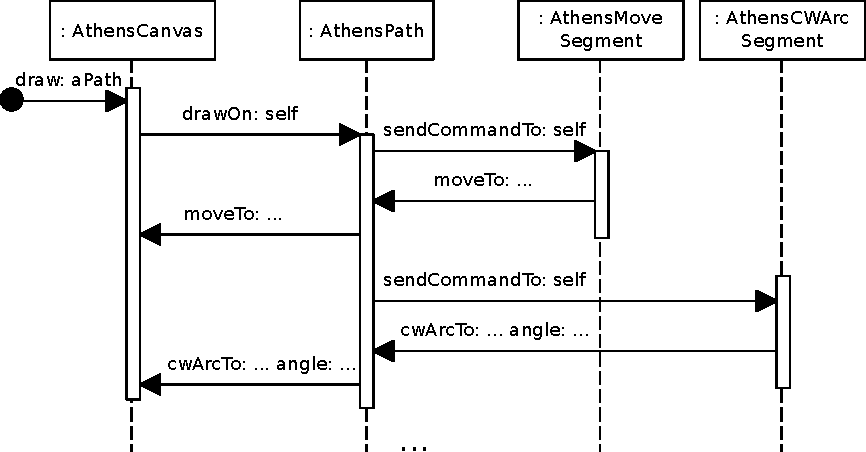
\includegraphics[width=\columnwidth]{athens_sequence.pdf}
    \caption{Drawing paths in Athens.}
    \label{fig:athens_sequence}
\end{figure}

\paragraph{Control Point Layer}
To make it easier to find drawing bugs, a control point layer is defined, which draws control points for all segments of a path. Control points are, for example, start and end points of lines and curves, or Bézier control points.

\begin{figure}[!htp]
\begin{lstlisting}[escapechar=!]
!\textbf{\texttt{\scriptsize moveTo: aPoint}}!
    self proceed: aPoint.
    self drawControlPoint: endPoint.

!\textbf{\texttt{\scriptsize drawControlPoint: aPoint}}!
    canvas pushStyle.
    canvas fillStyle: 'rgba(0, 0, 0, 0.5)'.
    canvas fillRect: (aPoint - (5@5) 
                        corner: 10@10).
    canvas popStyle.
\end{lstlisting}
\caption{Some partial methods for drawing control points.}
\label{fig:athens_partial}
\end{figure}

Figure~\ref{fig:athens_partial} shows some of the partial methods defined for the control point layer. \texttt{AthensPath} is the base class for these methods. ContextAmber allows programmers to add new methods to classes. For example, \texttt{drawControlPoint:} is not defined on \texttt{AthensPath}. By activating the control point layer on the path defined in Figure~\ref{fig:source_athens}, it is possible to show control points only for buttons, but not for other user interface elements.

\section{Implementation}
\label{sec:impl}
ContextAmber is our framework for context-oriented programming and used to evaluate and benchmark the concepts presented in this paper. It runs on top of Amber Smalltalk\footnote{\url{http://amber-lang.net}}, an implementation of the Smalltalk programming language that compiles to JavaScript.

\paragraph{Amber Smalltalk Object Model}
The Amber Smalltalk object model is minimalistic but follows closely the Smalltalk-80 object model. Every Smalltalk object is at the same time a JavaScript object. Instance-of and inheritance relationships are implemented using the JavaScript prototype hierarchy, i.e., every object has a prototype containing the instance methods for the corresponding class, and that object's prototype contains the instance methods of the super class. Message passing is implemented by JavaScript method calls, where colons in the selector are replaced with underscores.

When a Smalltalk method is compiled, its source code is first converted into an AST. Then a semantic analyzer performs checks and determines the type and scope of variables. The AST is then converted into an intermediate representation (IR) which is similar to the AST but distinguishes between local returns and non-local returns, for example. An IR tree can directly be transformed into JavaScript code.

ContextAmber performs method inlining on the AST level, making it possible to use the step-through debugger, which operates on the AST.

\paragraph{Layer Activation}
In ContextAmber, layers can be activated globally, within a certain scope, and for a single object. Since JavaScript is a single-threaded programming language, scoped layer activation can be treated like global layer activation\footnote{Amber Smalltalk does currently not support processes.}, as long as the effect is reversed once the control flow leaves the scope. As will be described in Section~\ref{sec:partial_method_inlining}, object-wise layer activation has far-reaching effects on method inlining, since different instances of the same class can have different layer compositions.

\begin{figure}[!htp]
    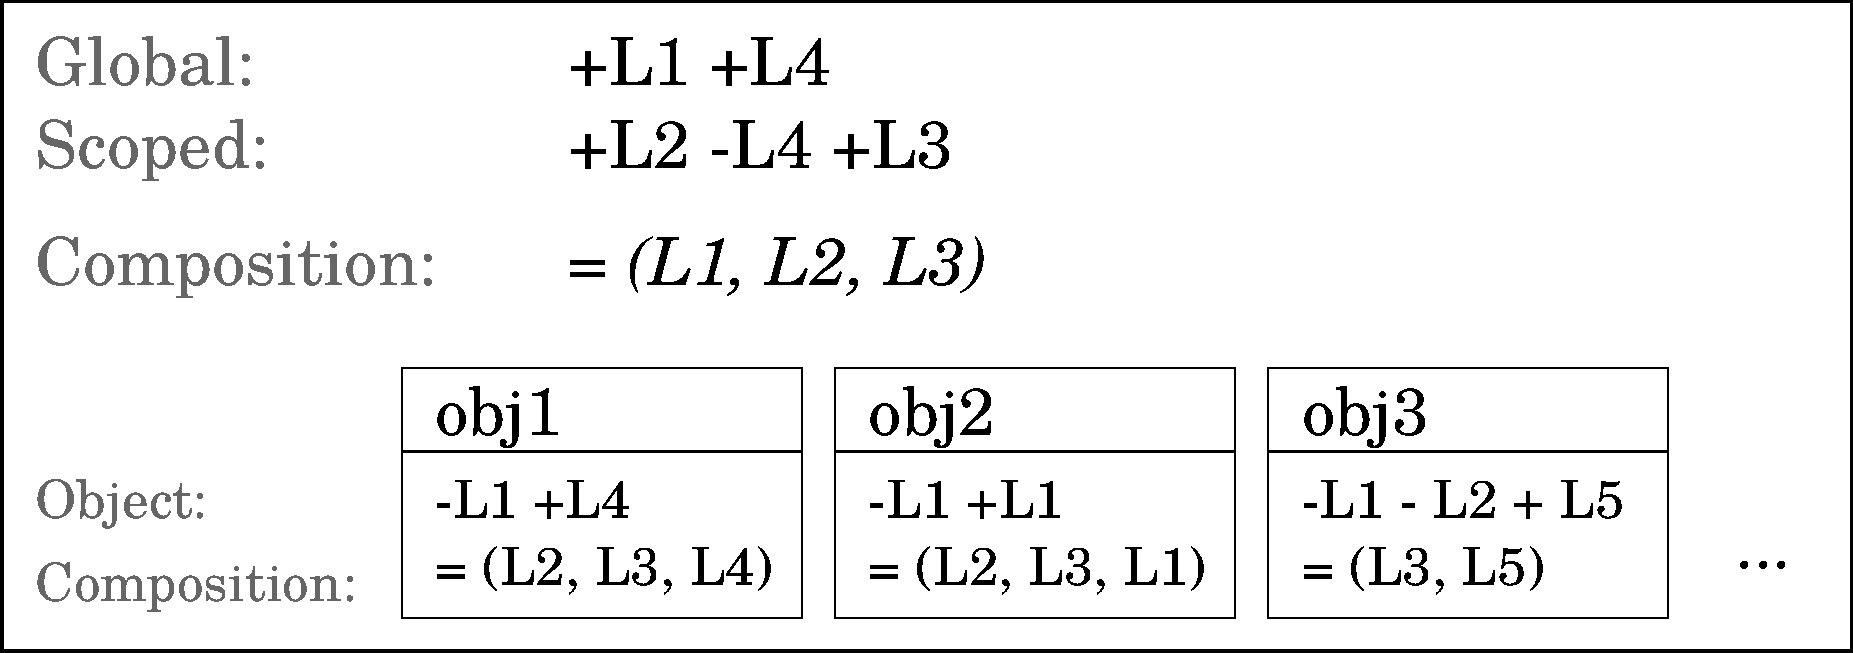
\includegraphics[width=\columnwidth]{layer_composition_calculation.pdf}
    \caption{Layer Composition Calculation in ContextAmber.}
    \label{fig:layer_composition_calculation}
\end{figure}

%\todo{Is there enough information given about layer composition computation?}
Figure~\ref{fig:layer_composition_calculation} shows how ContextAmber calculates an object's layer composition. Object-wise layer activation has a higher precedence than scoped layer activation, which has a higher precedence than global layer activation. In the rest of this work, we do not distinguish between global and scoped layer activation and refer to the global/scoped layer composition as the \emph{Global Layer Composition} (italic text in Figure~\ref{fig:layer_composition_calculation}).

\section{Partial Method Inlining}
\label{sec:inlining}
\label{sec:partial_method_inlining}
In this section, we discuss ContextAmber's two variants for inlining partial methods and their implications.

\subsection{Method Inlining}
ContextAmber hooks into the Amber compilation process and inlines methods on the AST level. A visitor looks for \texttt{proceed} sends and replaces them with a \texttt{value} send to a block closure containing the sequence of instructions of the next partial method in the current layer composition. This approach takes care of name clashes of temporary variables, as opposed to just copying the instructions without a block closure. Return statements in inlined methods must be modified, such that they don't cause the entire method to end but just return from the block closure (local return). 

\paragraph{Class-specific Method Inlining}
Inlined methods are stored on the prototype object for the class (like ordinary instance methods), i.e., the prototype that is shared by all instances of a class. This makes object-wise layer activation difficult, because ContextAmber might have to execute different inlined methods, depending on the object's layer composition.

%idea: class has multiple methods for different compositions

\paragraph{Instance-specific Method Inlining}
Inlined methods are stored as attributes on the object itself, allowing objects with different layer compositions to have their own inlined methods. This is usually not supported by Smalltalk, but, in JavaScript, every object can have its own methods. Some programming languages have similar concepts: for example, Ruby supports object-specific methods using singleton classes (eigenclasses). In some other programming languages, instance-specific method inlining can be harder to
implement using only metaprogramming facilities: an implementation would have to create a subclass containing the inlined method and change the object's class to that subclass. Alternatively, layered methods could be wrappers delegating calls to composition-specific item description objects~\cite{Coad:1992:OP:130994.131006}, or look up methods in a separate dictionary.

Instance-specific inlining can be faster than class-specific inlining because no new methods have to be installed when a method is called on objects with different layer compositions alternately. However, having too many different layer compositions can affect caching and VM optimizations and slow down the system. Future versions of ContextAmber might automatically decide whether to use class-specific or instance-specific inlining and adapt that decision during runtime if necessary. Currently, the programmer has to decide.

\subsection{Method Cache}
ContextAmber maintains a fixed-size method cache mapping layer compositions to inlined methods. Whenever an inlined method is requested, it is first looked up in the method cache. If an inlined method was not found in the cache, it is generated and added to the cache. Old inlined methods are evicted from the cache in a FIFO manner. 

Method caches make instance-specific method inlining feasible even with a large number of objects, because the same inlined method can be shared by multiple objects.

%TODO: effects on JIT compiler

\section{Inlined Method Invalidation}
\label{sec:invalidation}
\newcommand{\specialcell}[2][c]{%
\begin{tabular}[#1]{@{}c@{}}#2\end{tabular}}
\begin{figure*}[!htp]
\centering
\begin{tabular}{c|ccccc}
 & \specialcell{instance- \\ specific} & \specialcell{class- \\ specific} & \specialcell{instance \\ space overhead} & \specialcell{update header \\ runtime overhead\footnotemark} & \specialcell{composition change \\ runtime overhead} \\
\hline
Comparing signatures & \ding{51} & \ding{51} & no overhead & \specialcell{compute composition \\ compare signature} & no overhead \\ \hline
Caching signatures & \ding{51} & \ding{51} & \specialcell{boolean field \\ integer field \\ string field} & \specialcell{compare dirty bit \\ compare version \\ (compare signature)} & \specialcell{object: set dirty bit \\ global: increment version} \\ \hline
\specialcell{Detecting comp. changes \\ without signatures} & \ding{51} & \ding{55} & no overhead & \specialcell{compare signature} & \specialcell{object: delete method \\ global: compute global \\ composition signature} \\ \hline
\specialcell{Method generation \\ on composition change} & \ding{51} & \ding{55} & no overhead & no overhead & \specialcell{compute composition \\ generate mult. methods}
\end{tabular}

When using instance-specific method inlining, an additional method object is stored per instance\footnotemark.
\caption{Comparison of techniques for layered method invalidation and inlining.}
\label{fig:invalidation_comparison}
\end{figure*}

Method inlining improves the execution performance of layered methods; however, the overhead of iterating through the layer composition and performing a number of partial method dispatches is just shifted to another point of time. Whenever we inline a method, we are speculating that the layer composition will remain constant for a while, but we have to validate that assumption at some point. Once it becomes apparent that an inlined method is no longer up to date, it is invalidated, which causes the inlined method to replace itself with an updated version when it is called again. In this section, we discuss how and when ContextAmber invalidates inlined methods (see Figure~\ref{fig:invalidation_comparison} for an overview).

\subsection{Method Invalidation Reasons}
The following list gives an overview of the events that can cause an inlined method to be invalidated.

\begin{compact_item}
    \item \emph{Adding/removing a Partial Method.} If a partial method is added or removed for a layer that is currently active, ContextAmber might have to add or remove that partial method to corresponding inlined layered methods.
    \item \emph{Calling a Method on a Different Object.} With object-wise layer activation, two different instances of the same class can have different layer compositions and, therefore, different inlined layered methods. A layered method that is inlined for the entire class has to invalidate itself when it is invoked on an object having a different layer composition than the one it was created for.
    \item \emph{Layer Composition Change.} Inlined methods can be become outdated when a layer is activated or deactivated.
\end{compact_item}

\subsection{Invalidation on Invocation}
Every inlined method contains an \emph{update header} that determines if the method is up to date. If this check is positive, then the execution of the inlined method continues. Otherwise, a new version of the inlined method with the current layer composition is generated, installed, and executed. In this subsection, we give an overview of different update headers and when they are suitable.

\paragraph{Comparing Composition Signatures}
Every layer has a unique integer identifier. A layer composition can be uniquely represented by its layer composition signature (i.e., fingerprint~\cite{Krahn:2012:ELA:2223947.2223971}): a concatenation of the layers' IDs and separator characters. The most basic update header is shown in Figure~\ref{fig:update_unoptimized}.

\begin{figure}[!htp]
    \centering
    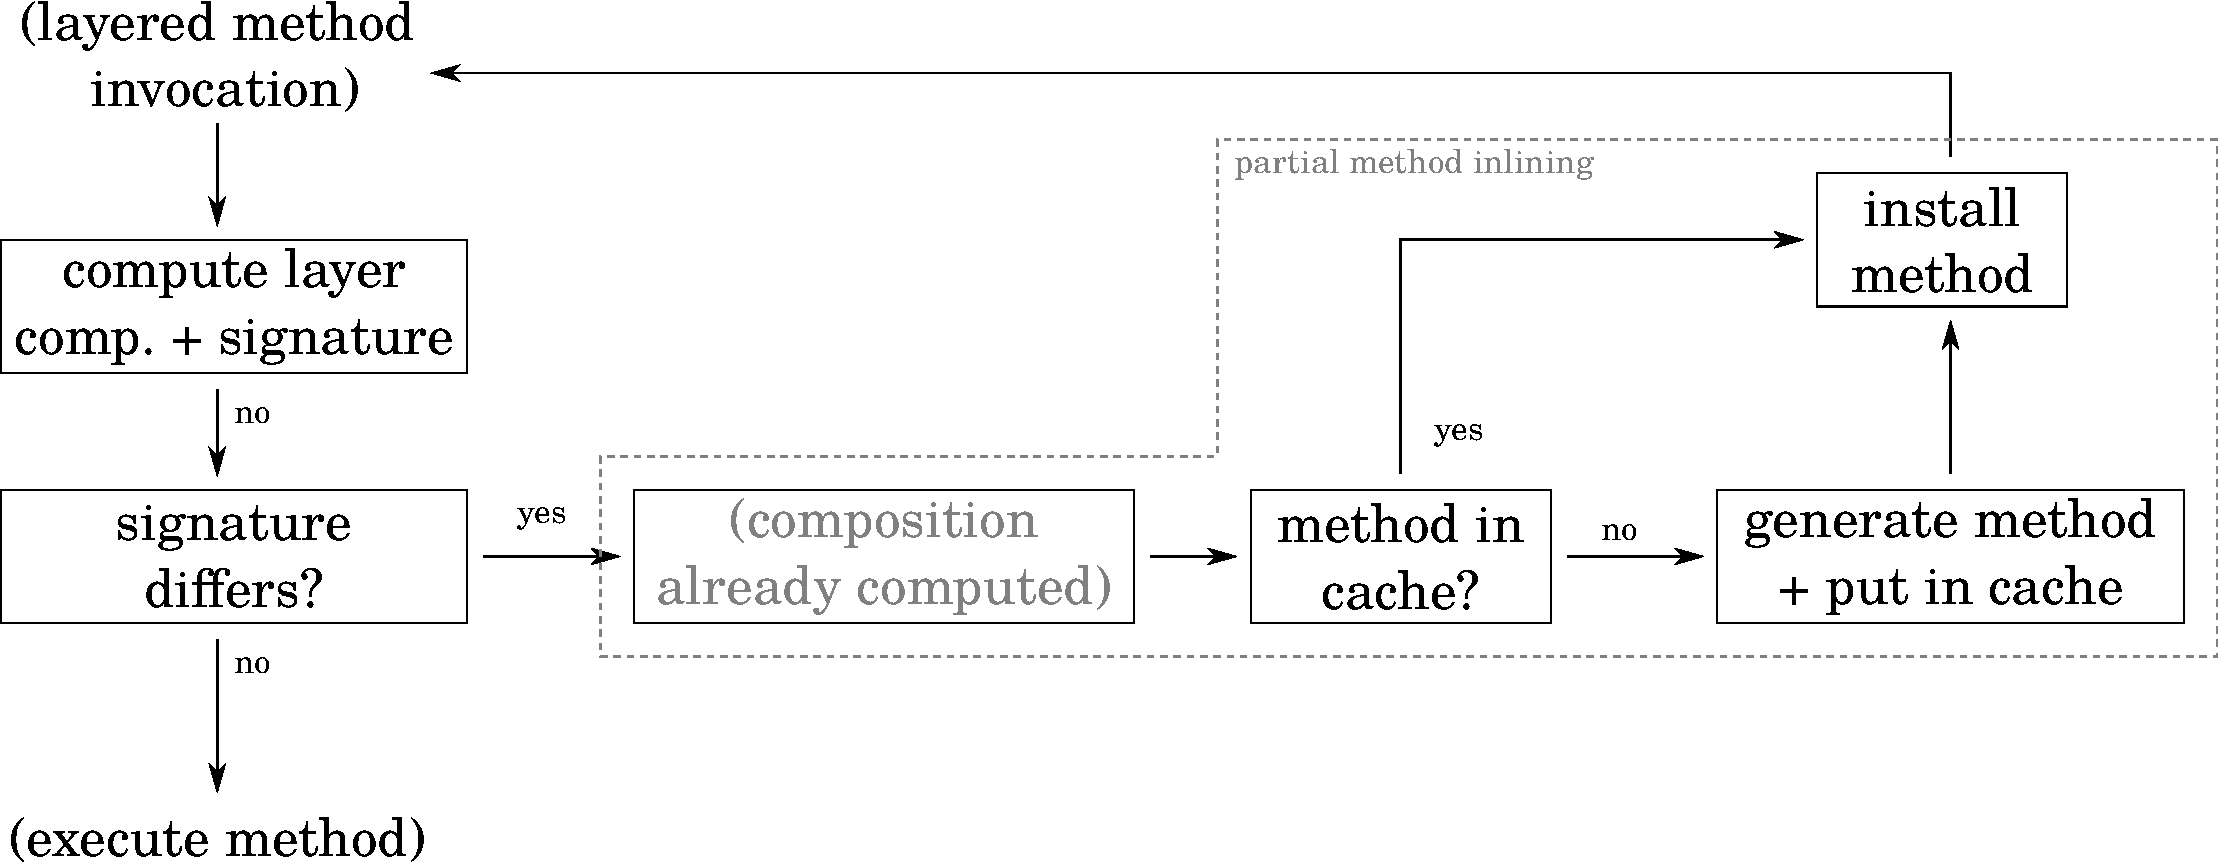
\includegraphics[width=\columnwidth]{update_header_unoptimized.pdf}
    \caption{Update header for comparing layer composition signatures.}
    \label{fig:update_unoptimized}
\end{figure}

When an inlined layered method is invoked, the update header computes the receiver's layer composition and its layer composition signature and compares it with the layer composition signature at the point of time when the inlined method was generated. That value is hard-coded as a string literal in the update header's source code. If the signature values differ, then a new inlined method is created, installed, and called. A method cache is used to cache inlined methods and avoid unnecessary code generation.

\footnotetext[6]{We consider the average case where the layer composition was not changed (or invariant layer composition change sequences).}
\footnotetext{Method caches make it easy to share the same method object among multiple instances.}

\paragraph{Caching Composition Signatures}
The update header in Figure~\ref{fig:update_unoptimized} has to compute the current layer composition every time the method is invoked. ContextAmber can speed up this step by caching layer composition signatures on a per-object basis. Recalculating the signature whenever a composition change is made is not suitable, because a global layer composition change can affect a large number of objects whose signatures would have to be updated (Figure~\ref{fig:layer_composition_calculation}). Instead, the composition signature becomes \emph{outdated} whenever the layer composition is changed globally or on a per-object basis: in the former case, a version number is incremented on all base classes affected by the layer, indicating that a change was made that affects all of its instances. In the latter case, the object is marked as dirty, indicating that only the layer composition for that single object changed. The update header uses the cached composition signature if the receiver is not marked dirty and its version number equals its class' version number. Otherwise, the layer composition is recomputed, along with its signature (Figure~\ref{fig:update_header_caching}).

\begin{figure}[!htp]
    \centering
    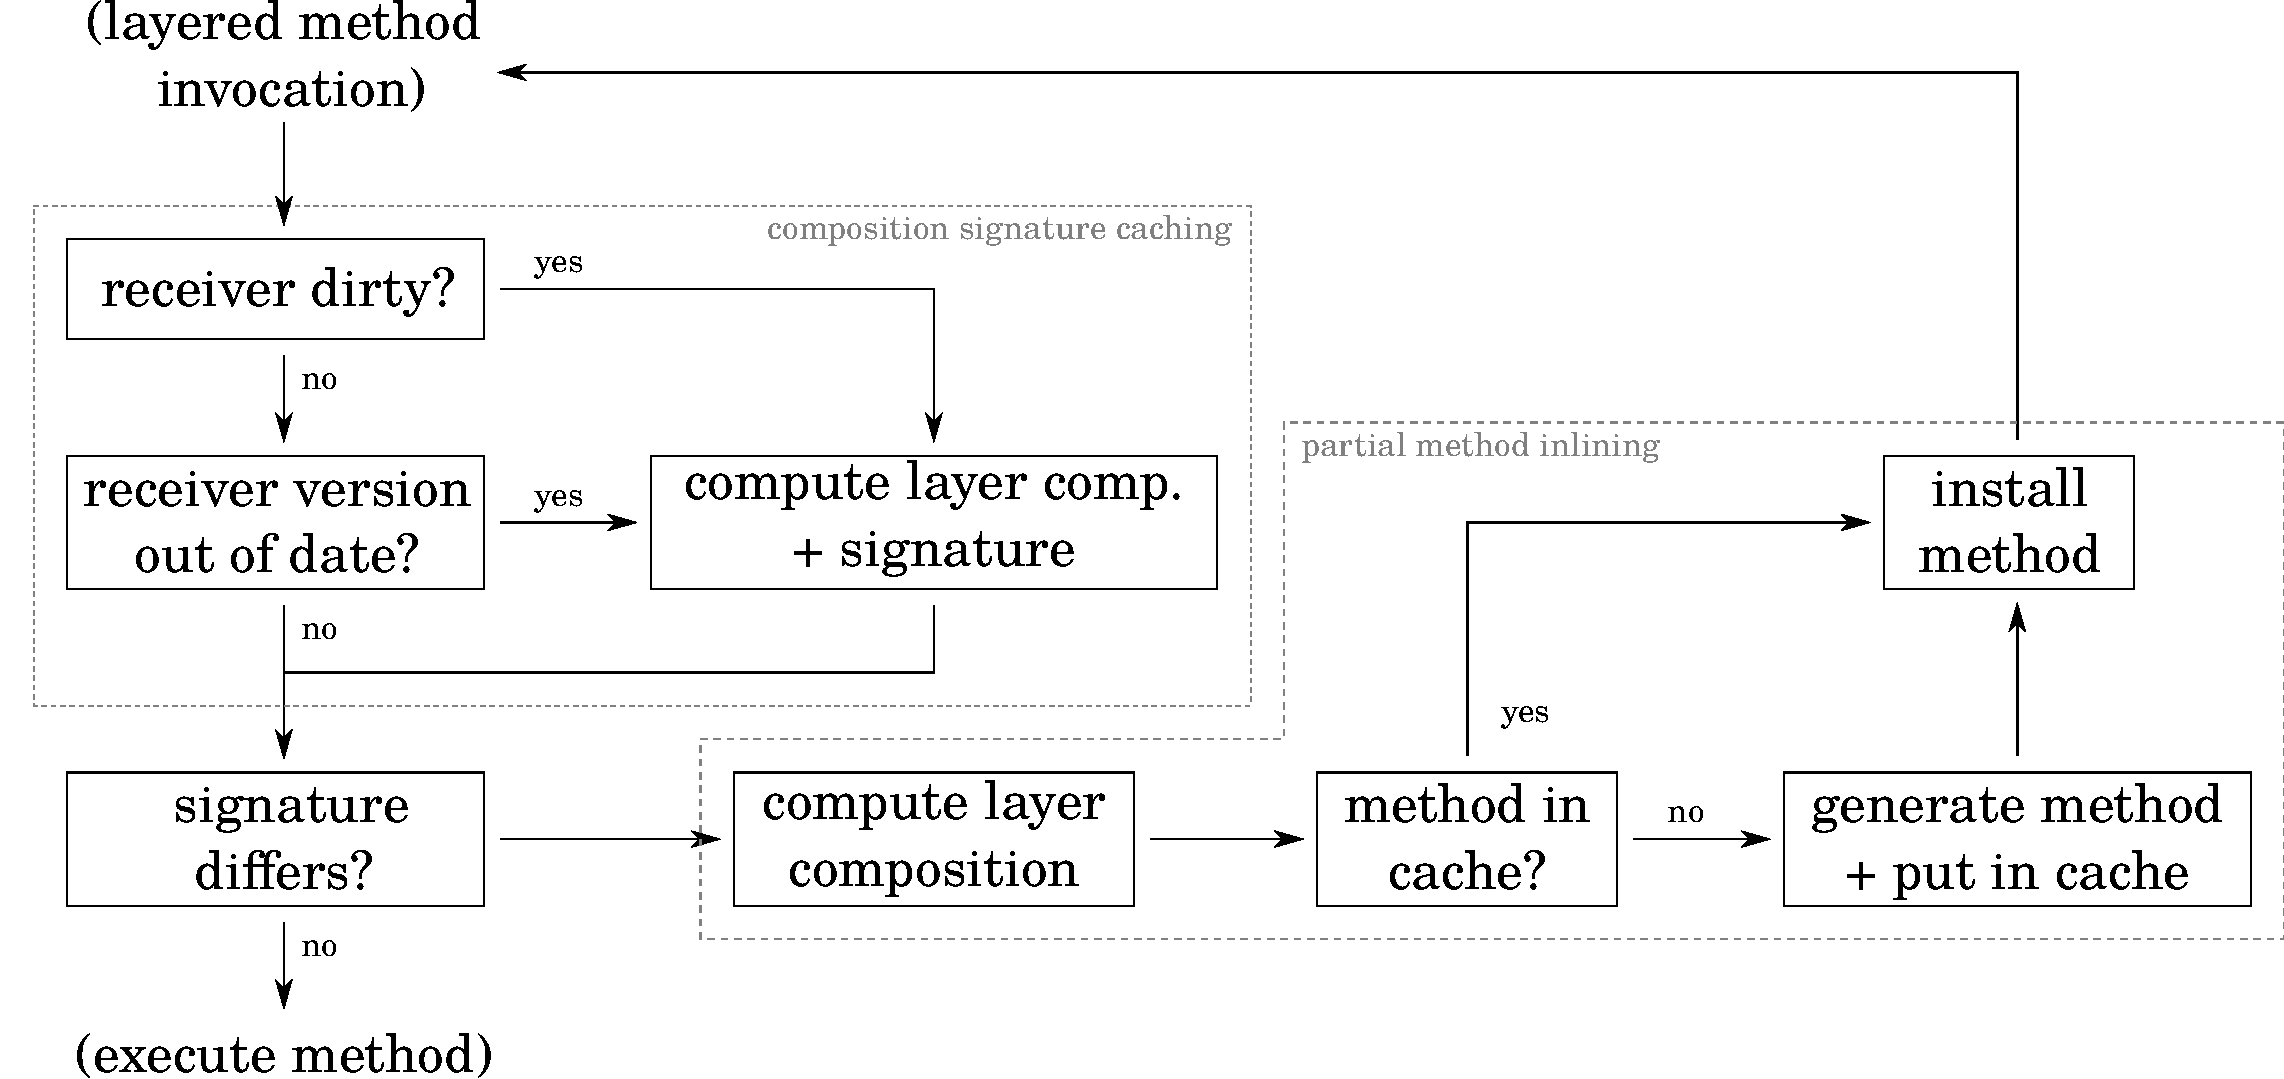
\includegraphics[width=\columnwidth]{update_header_class_wide.pdf}
    \caption{Update header for caching layer composition signatures.}
    \label{fig:update_header_caching}
\end{figure}

In total, ContextAmber stores three additional fields on every object with a layered method\footnote{These fields are stored as JavaScript object attributes that are not visible from the Smalltalk side and do not interfere with Smalltalk code.}: the cached layer composition signature (string), the version number (integer) of the object's class at the point of time when the layer signature was cached, and a dirty bit (boolean). These three fields are refreshed whenever the composition signature is recomputed.

Note, that composition signature is both hard-coded in the method source code and stored as a field on every object having layered methods. These two values are being compared in the update header. ContextAmber uses this technique for class-specific method inlining.

\paragraph{Detecting Composition Changes without Signatures}
The update header in Figure~\ref{fig:update_header_caching} has to compare composition signatures because a different inlined method might have to be installed even if there are no changes to the layer composition: if a class-specific inlined method is invoked on objects with different layer compositions. Instance-specific inlined method do not have to be invalidated in that case, because every object has its own method (Figure~\ref{fig:update_header_detecting}).

\begin{figure}[!htp]
    \centering
    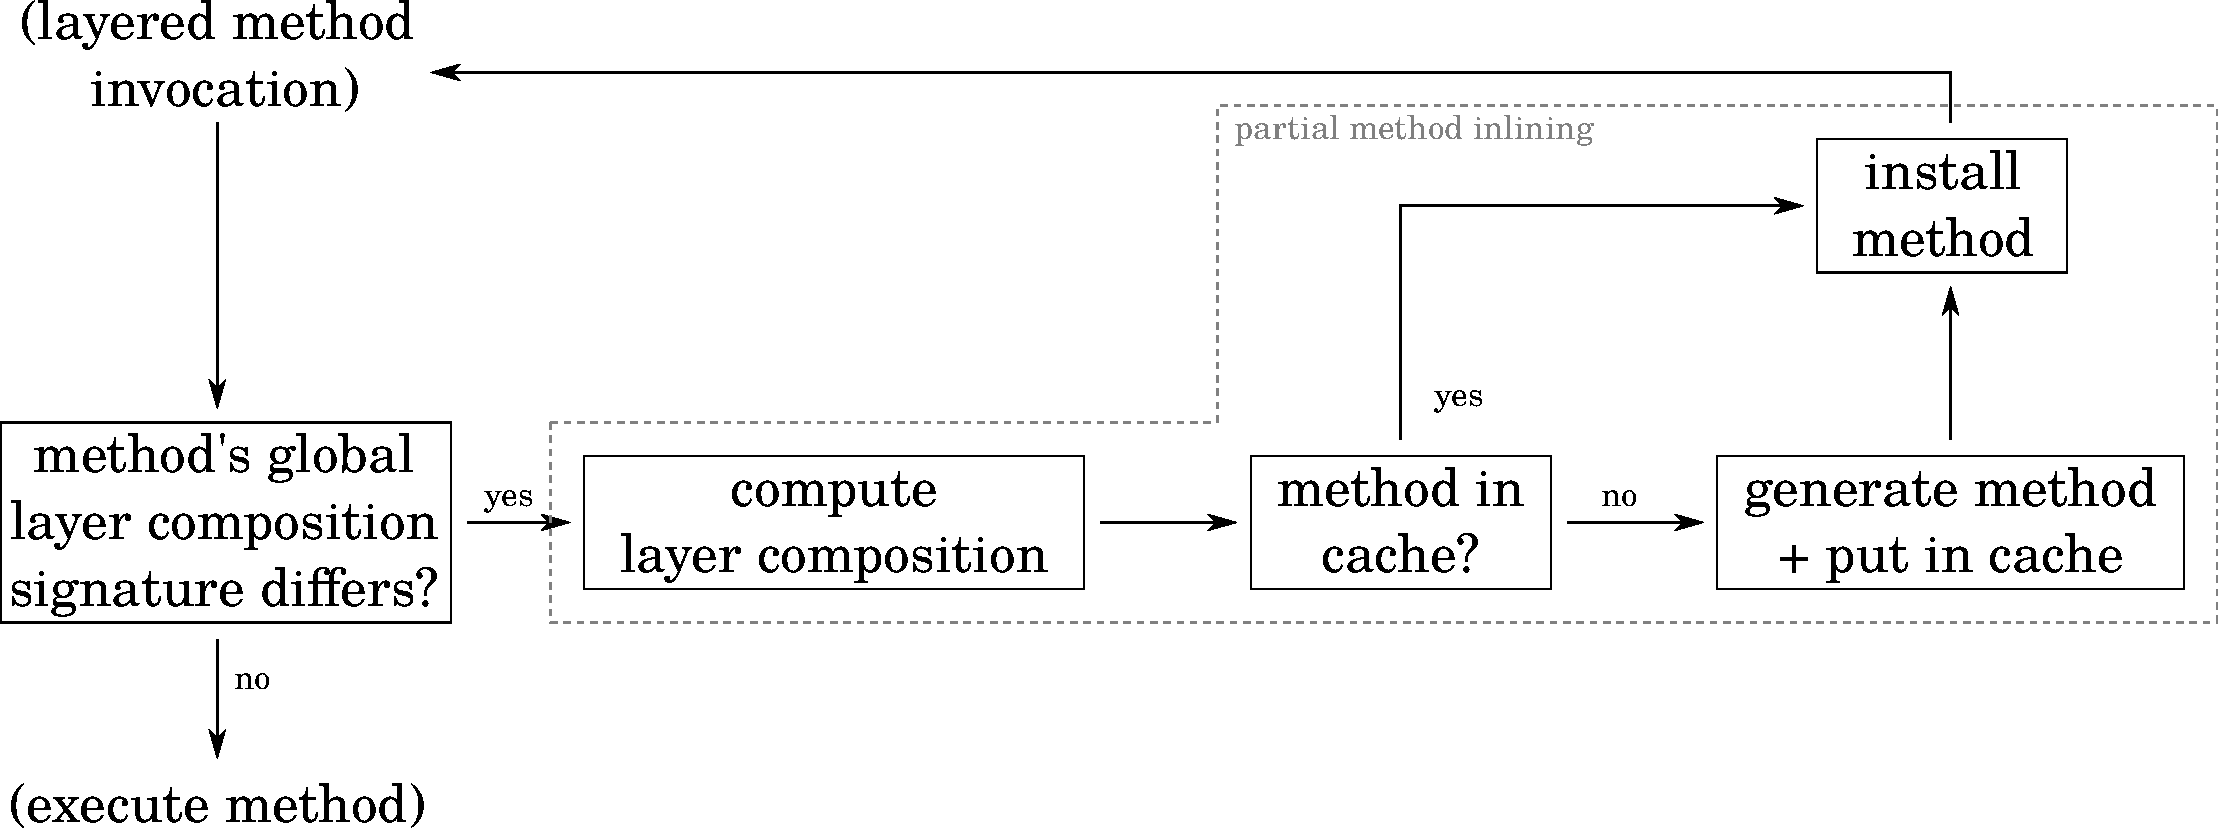
\includegraphics[width=\columnwidth]{update_header_detecting.pdf}
    \caption{Update header for detecting layer composition changes without comparing layer composition signatures.}
    \label{fig:update_header_detecting}
\end{figure}

If the layer composition is changed for an object, ContextAmber simply removes affected inlined methods from the object. The object's class has corresponding instance methods that will generate and install a new inlined method on the object. No dirty bit is needed. 

If the layer composition is changed globally, ContextAmber updates the global layer composition signature for all affected method objects stored in the class' method dictionary, i.e., it updates an instance variable on all affected \texttt{CompiledMethod} objects\footnote{Only layers
having a corresponding partial method are part of that signature.}. The update header has the global layer composition signature at the time of inlining hard-coded as a string and compares it with the signature stored in the class' method object. Note, that invariant global layer composition change sequences, i.e., sequences of global layer composition changes that do not change the global layer composition (e.g., activating and deactivating a layer globally), do not invalidate a method, because the
global layer composition signature stays the same. ContextAmber uses this technique for instance-specific method inlining.

\section{Benchmarks}
\label{sec:bench}
As a benchmark, we are rendering a simplified version of the GhostScript Tiger (Figure~\ref{fig:gs_tiger}), consisting of 31 paths and 211 segments in total. If the control point layer is activated, each segment draws at least one control point.

\begin{figure}[t]
        \centering
        \subfloat[Without layers.]{
\includegraphics[width=0.45\columnwidth]{tiger_original.pdf}}
        \hfill
        \subfloat[Control point layer.]{
\includegraphics[width=0.45\columnwidth]{tiger_control_resized.png}}
    \caption{GhostScript Tiger rendering with Athens.}
    \label{fig:gs_tiger}
\end{figure}

Figure~\ref{fig:rendering_runtime} shows the runtime for rendering the tiger 1000 times in a loop\footnote{Benchmarks were run on a MacBook Pro with an i7-4558U CPU and 16~GB RAM, using Chrome 41.0.2272.118 (64-bit). We used \url{git@github.com:matthias-springer/cop-ContextAmber.git} at commit \texttt{0006c8b997}.}. The runtime for the first frame is higher than the average runtime, because this is when an inlined method is created for the first time. The runtime increases if new methods have to be installed: \emph{control point layer (mixed)} denotes the case where the control point layer is active only on 50\% of the path objects (on every second one). If method caching is enabled, its class-specific case remains reasonably fast because inlined methods with and without the control point layer are cached; subsequent frame renderings with instance-specific inlining are already fast without caches, because no new methods have to be installed. However, rendering the first frame benefits from method caches even then, because only two methods are then generated and cached (with/without layer). The benchmarks in Figure~\ref{fig:rendering_runtime} do not change the layer composition during rendering. 

\begin{figure}[t]
    \centering
    \subfloat[Avg. frame rendering runtime (excluding first frame).]{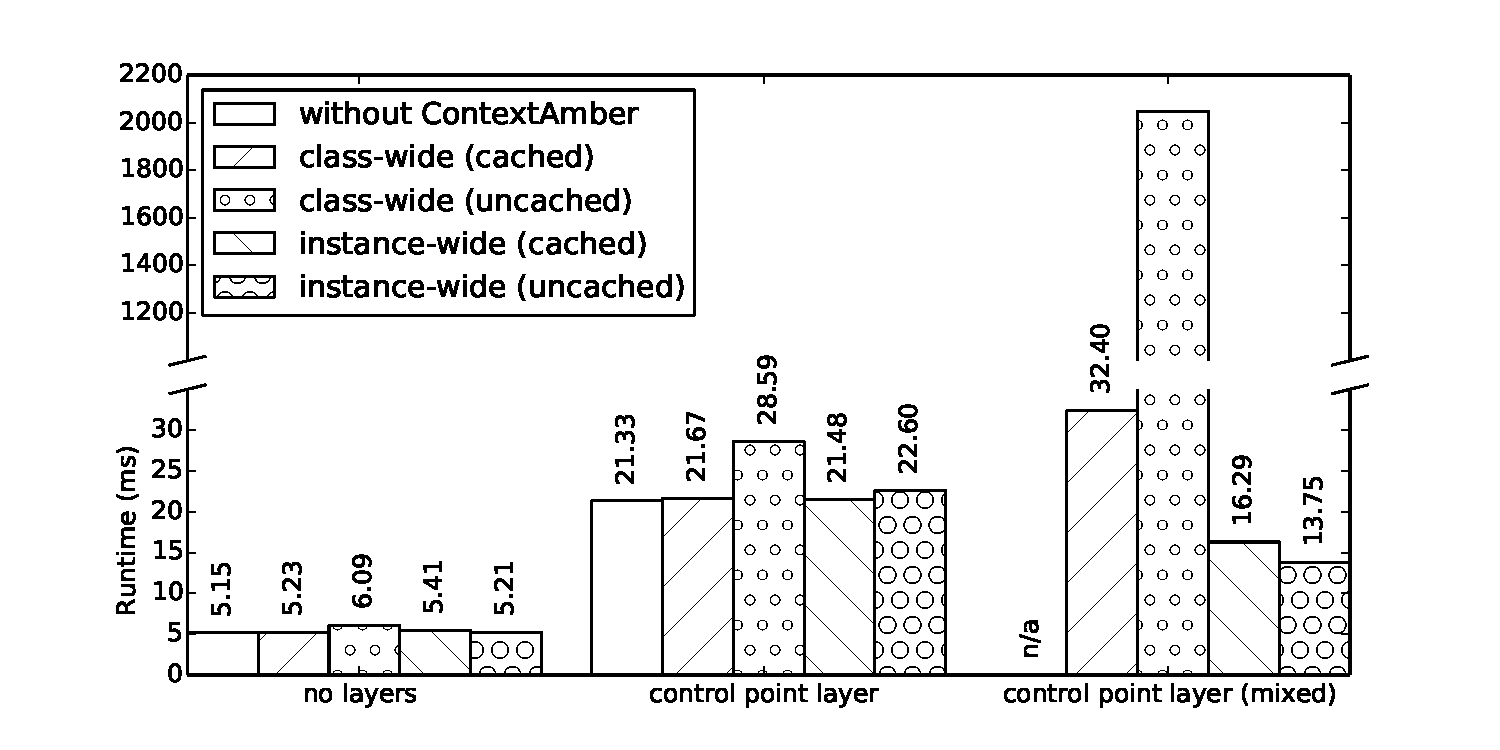
\includegraphics[width=\columnwidth]{plot_bench_frames.pdf}} \\
    \subfloat[First frame rendering runtime.]{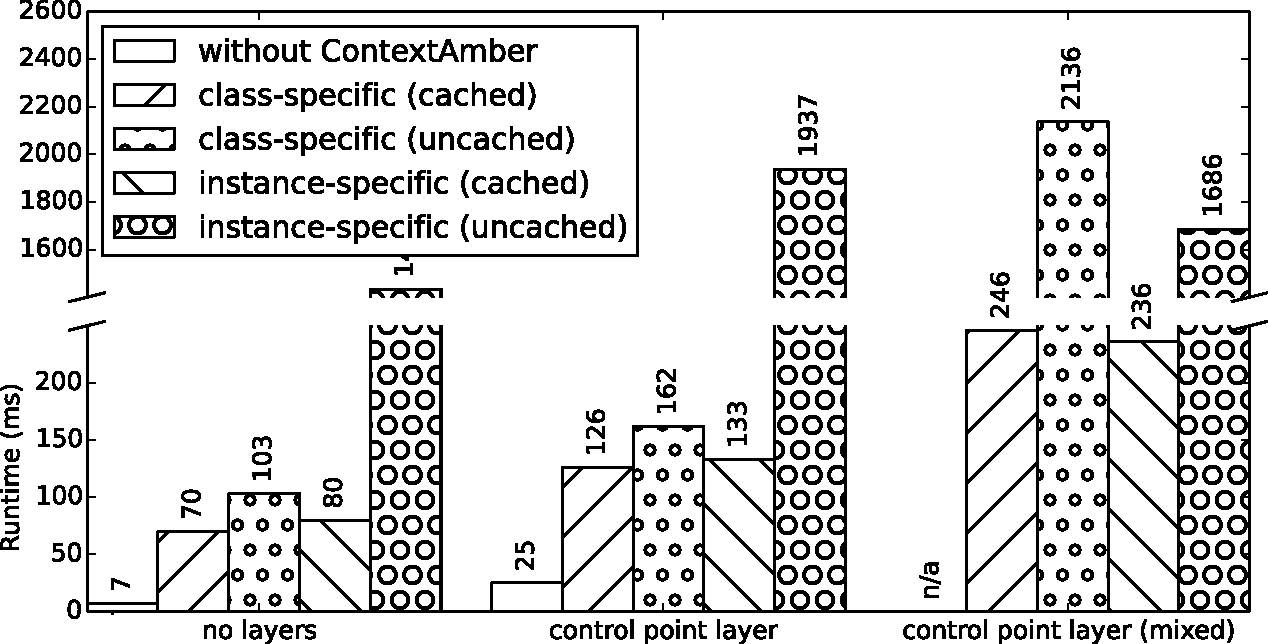
\includegraphics[width=\columnwidth]{plot_bench_first_frame.pdf}}
%    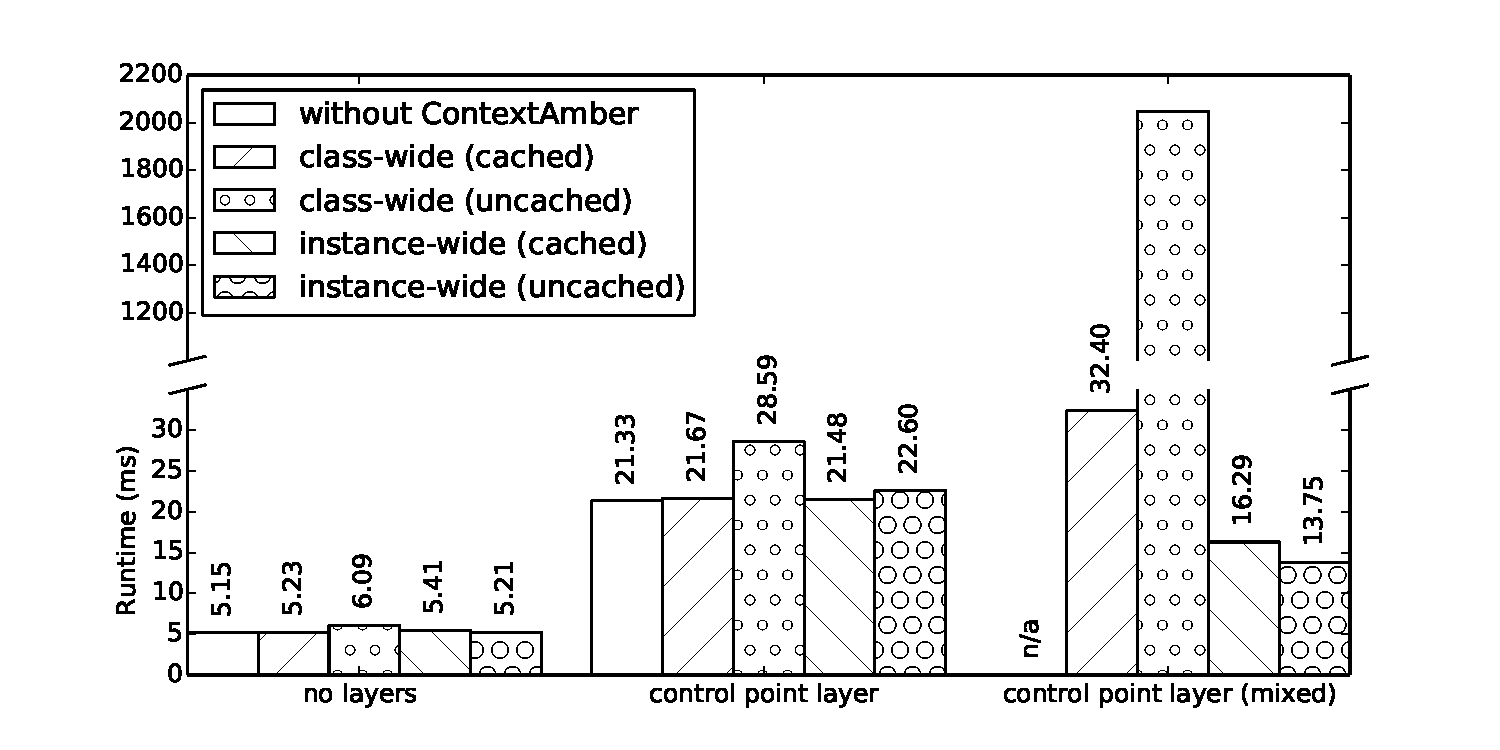
\includegraphics[width=\columnwidth]{plot_bench_frames.pdf}
    \caption{Tiger rendering runtime in milliseconds.}
    \label{fig:rendering_runtime}
\end{figure}

Figure~\ref{fig:activation} shows the average runtime for activating and immediately deactivating a layer again. Activating a layer object-wise is slow, because ContextAmber stores layer activation statements in a custom data structure consisting of two stacks: one stack for activations, one stack for deactivations. This is not necessary for global layer activation, because it has the lowest precedence: it is sufficient to store one list of currently
activated layers. Instance-specific inlining is slower than class-specific inlining because ContextAmber deletes inlined methods (object) or recomputes the global layer composition signature (global) instead of marking the object dirty or increasing a version number, respectively.

\begin{figure}[t]
    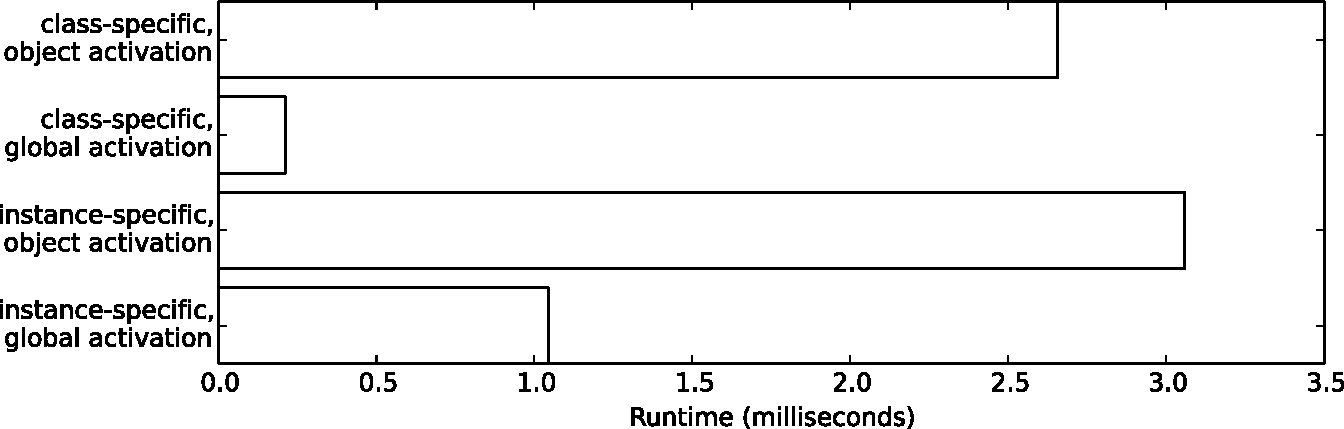
\includegraphics[width=\columnwidth]{activation_ms.pdf}
    \caption{Runtime for activating/deactivating a layer.}
    \label{fig:activation}
\end{figure}

\section{Related Work}
ContextJS is a COP implementation for JavaScript~\cite{Lincke:2011:OIC:1998661.1998804}. It relies solely on metaprogramming facilities. It is similar to ContextAmber in a sense that both run on JavaScript. It inlines \texttt{proceed} calls in the same way ContextAmber does, and adds an update header to the beginning of every inlined method checking the object's cached layer composition signature; caching is, however, not supported for object-wise layer activation because every object can provide its own method for computing the stack of activated layers~\cite{Krahn:2012:ELA:2223947.2223971}.

ContextS is a COP implementation for Squeak~\cite{Hirschfeld:2007:ICP:1462618.1462629}. Layers are represented by classes and their methods contain the name of the base class, the selector, and the partial method as a block closure in the source code. In ContextAmber, partial classes containing partial methods are associated with layer classes in a many-to-many relationship.

ContextL is a performance-efficient COP implementation for CLOS. Layers are internally represented by classes and layer compositions are cached classes that inherit from (multiple) layer classes: the topmost layer class and a layer composition class for the rest of the layer composition, where the former one takes precendence over the latter one~\cite{Costanza:2006:ELA:2111746.2111753}.

\section{Future Work}
The ideas presented in this work are based entirely on metaprogramming. Changing the language interpreter or virtual machine, however, allows for a variety of different implementations. Future work might focus on making polymorphic inline caches~\cite{Holzle:1991:ODO:646149.679193} aware of layer compositions: the invoked method could be determined based on the polymorphic type of the receiver and its layer composition signature.

Another optimization could make systems, that do already perform aggressive method inlining, aware of layer compositions and \texttt{proceed} calls. Basically, \texttt{proceed} calls could be treated as a special form of method calls with a different method lookup procedure in the interpreter. Together with special guard clauses, a \texttt{proceed} call could look as ordinary to the inliner as any other method call. Partial Evaluation in Truffle~\cite{Wurthinger:2013:OVR:2509578.2509581} is an example of a very aggressive form of method inlining that could be made aware of layer compositions: it continues inlining methods until it encounters a statement that tells it to stop inlining.

Future work could also investigate subclassing of partial classes.

\section{Summary}
We presented our COP implementation ContextAmber for Amber Smalltalk. ContextAmber reduces the runtime performance overhead of context-oriented programming by caching and executing inlined methods specific to a certain layer composition. ContextAmber can inline methods on a per-instance and on a per-class basis, and depending on the use case, the programmer can choose which one to use. ContextAmber is implemented using metaprogramming facilities, restricting our range of optimizations.
Future work might investigate optimizations on the virtual machine level.

%
% The following two commands are all you need in the
% initial runs of your .tex file to
% produce the bibliography for the citations in your paper.
\bibliographystyle{abbrv}
\bibliography{cop2015}  % sigproc.bib is the name of the Bibliography in this case
% You must have a proper ".bib" file
%  and remember to run:
% latex bibtex latex latex
% to resolve all references
%
% ACM needs 'a single self-contained file'!
%
%APPENDICES are optional
%\balancecolumns
\balancecolumns
% That's all folks!
\end{document}
